\section{Introduction}

TV archives maintained by national institutions such as the French INA, the Netherlands Institute for Sound \& Vision, or the British Broadcasting Corporation are rapidly growing in size. The need for applications that make these archives searchable has led researchers to devote concerted effort to developing technologies that create indexes.

Because human nature leads people to be very interested in other people.
Indexes that represent the location and identity of people in the archive are indispensable for searching archives.
%
To this end, started in 2011, the REPERE challenge aimed at supporting research on multimodal person recognition~\cite{BERNARD--SLAM--2013, KAHN--CBMI--2012}. Its main goal was to answer the two questions \emph{``who speaks when?''} and \emph{``who appears when?''} using any available source of information (including pre-existing biometric models and person names extracted from text overlay and speech transcripts). 
%
Thanks to this challenge and the associated multimodal corpus~\cite{GIRAUDEL--LREC--2012}, significant progress was achieved in either supervised or unsupervised multimodal person recognition~\cite{BECHET--INTERSPEECH--2014, BREDIN--ODYSSEY--2014, BREDIN--IJMIR--2014, GAY--CBMI--2014, POIGNANT--ASLP--2015, POIGNANT--INTERSPEECH--2012, POIGNANT--MTAP--2015, ROUVIER--CBMI--2014}.

However, when the content is created or broadcast, it is not always possible to predict which people will be the most important to find in the future and biometric models may not yet be available at indexing time The goal of this task is thus to address the challenge of indexing people in the archive under real-world conditions, \emph{i.e.} when there is no pre-set list of people to index.
%
This makes the task completely unsupervised (\emph{i.e.} using algorithms not relying on pre-existing labels or biometric models).
%
In order to successfully tag people with the correct identities, one must find a way to assign a name correctly to a presence of the corresponding person, then that name must also be propagated to all the shots during which that person appears and speaks. For this purpose, there are 3 possible approaches:
%
Clustering is common baseline, but there are more and more methods with the rise of new systems.
%
\begin{compactitem}
\item{Clustering-based naming: Face/speech tracks are first aggregated into homogeneous clusters according to person identities. Then each clusters is tagged with the most probable person name.}
\item{Verification-based name propagation: A person name is first assigned to the most probable face/speech track. The name is then propagated to all face/speech tracks which are verified to have the same identity.}
\item{Graph-based name propagation: A graph is built with a face/speech track as a node and weight of edges is the similarity. Some nodes are initially tagged with the names. Names are then propagated along the edges within the graph.}
\end{compactitem}

There are several problems related to these approaches such as face / speech representation, person diarization, or audio-visual verification. Each of these problems has been well studied within its respective context~\cite{recog,veri,rep}. 
%
However, these approaches have never been fully investigated and compared as whole systems in the large-scale multimedia indexing context before. In this paper, the authors aim to investigate all these approaches with variations in their components using real world datasets from TV news. 
%
To emphasize on the unsupervised nature of real world applications, we applied these approaches on a large scale multimedia dataset associated to the ``Multimodal Person Discovery in Broadcast TV'' task~\cite{POIGNANT--MEDIAEVAL--2015,bredin2016mediaeval}. In this task, participants are provided with a collection of TV broadcast recordings pre-segmented into shots. Each shot $s \in \shots$ has to be automatically tagged with the names of people both speaking and appearing at the same time during the shot.
%
The benchmarking results allow us to thoroughly analyse all 3 approaches to understand their pros and cons. Thus, we can draw meaningful lessons for good practice in large-scale person discovery in broadcast news.

\subsection{MediaEval Person Discovery challenge}

\mypartitle{Task overview.} Participants are provided with a collection of TV broadcast recordings pre-segmented into shots.
Each shot $s \in \shots$ has to be automatically tagged with the names of people both speaking and appearing at the same time during the shot: this tagging algorithm is denoted by $\hypLabels : \shots \mapsto \mathcal{P}(\hypNames)$ in the rest of the paper.

As last year, the list of persons is not provided \emph{a priori}, and person biometric models (neither voice nor face) can not be trained on external data in the primary runs. The only way to identify a person is by finding their name $n \in \hypNames$ in the audio (\emph{e.g.} using speech transcription -- ASR) or visual (\emph{e.g.} using optical character recognition -- OCR) streams and associating them to the correct person. This makes the task completely unsupervised (\emph{i.e.} using algorithms not relying on pre-existing labels or biometric models). The main novelty of this year task is that participants may use their contrastive run to try brave new ideas that may rely on any external data, including textual metadata provided with the test set.

Because person names are detected and transcribed automatically, they may contain transcription errors to a certain extent (more on that later in Section~\ref{sec:metric}). In the following, we denote by $\refNames$ the set of all possible person names in the universe, correctly formatted as \texttt{firstname\_lastname} -- while $\hypNames$ is the set of hypothesized names.

\begin{figure}[!htb]
 \centering
 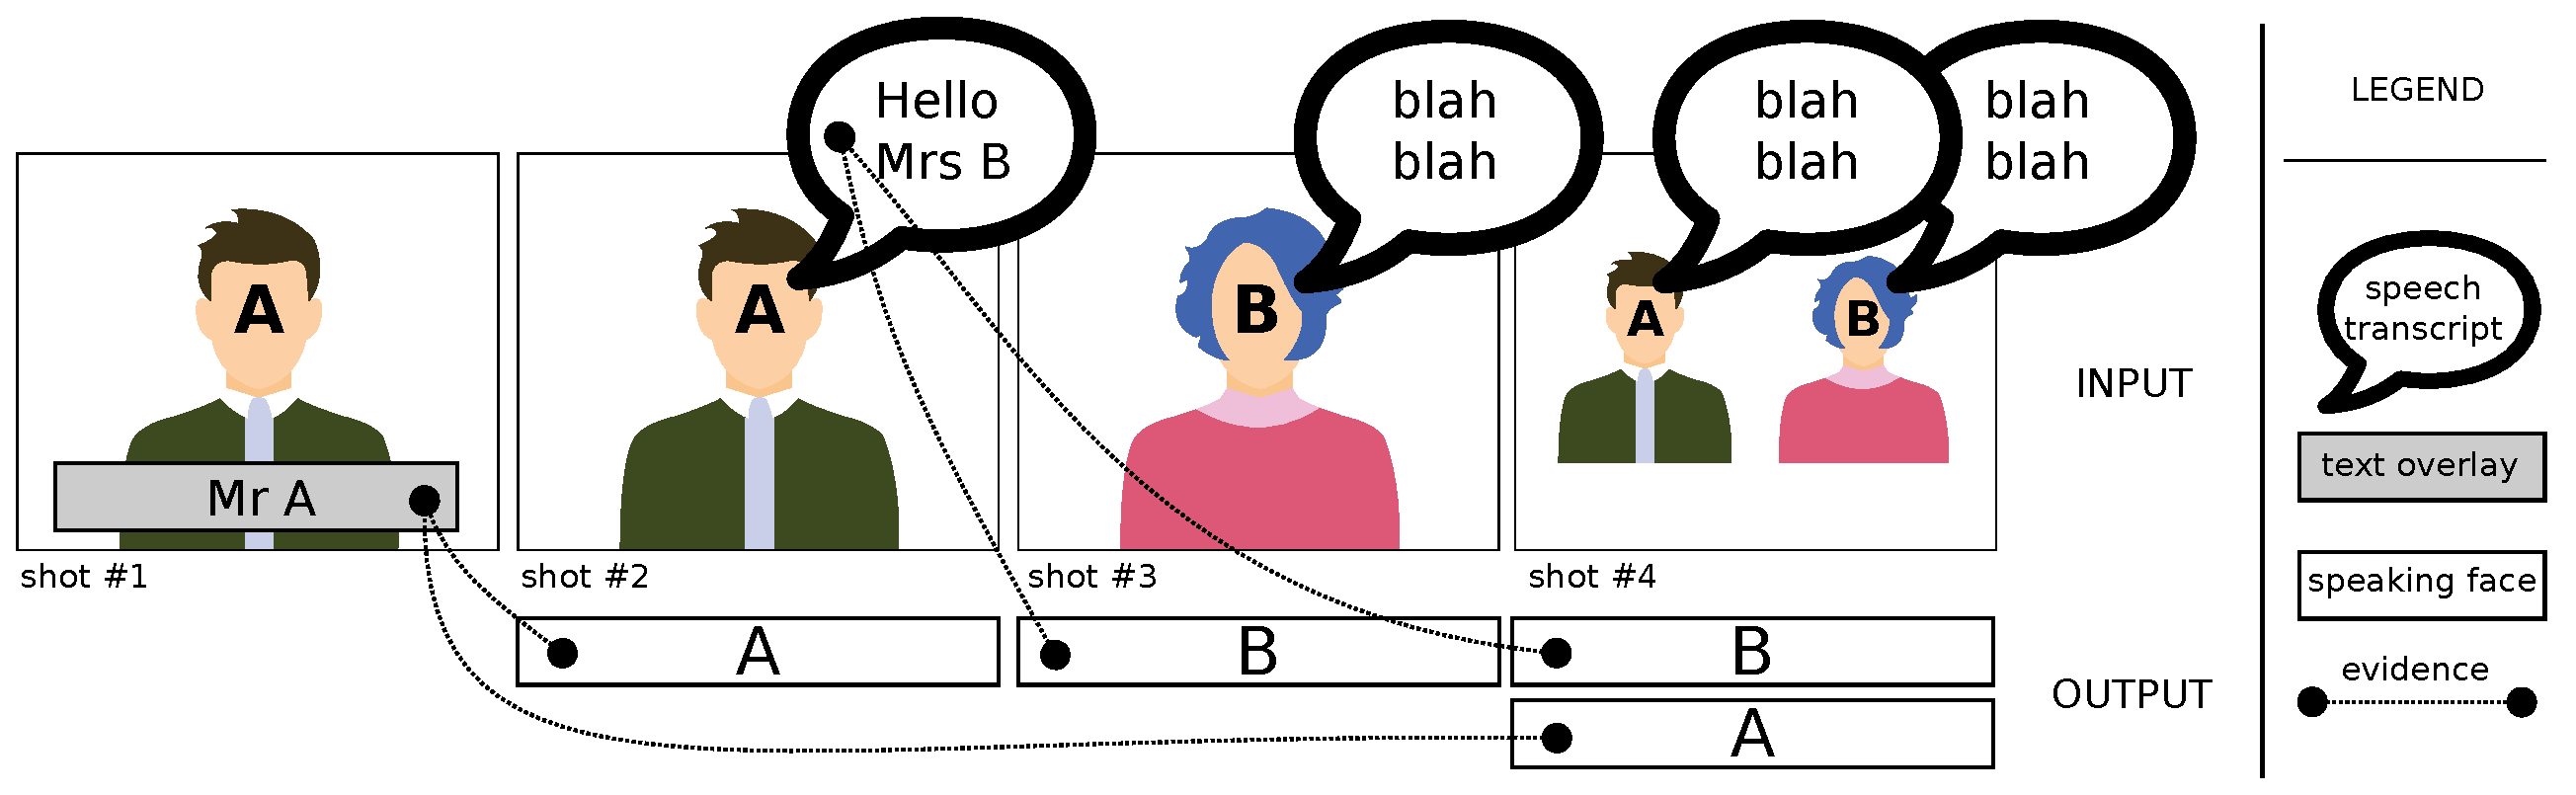
\includegraphics[width=1.\linewidth]{evidence.pdf}

 \caption{For each shot, participants have to return the names of every speaking face. Each name has to be backed up by an evidence.}
 \label{fig:evidence}
\end{figure}

\mypartitle{Datasets and annotation.} The test set is divided into three datasets: INA, DW and 3-24. The INA dataset contains a full week of broadcast for 2 TV channels for a total duration of 90 hours in French. The DW dataset~\cite{EUMSSI} is composed of video downloaded from Deutsche Welle website, in English and German for a total duration of 50 hours. The last dataset contains 13 hours of broadcast from 3/24 Catalan TV news channel. Each shot has been tagged with the names of people who appear and speak within that shot.

\mypartitle{Metrics.} The task is evaluated indirectly as an information retrieval task, using the folllowing principle.
%
For each query $q \in \queries \subset \refNames$ (\texttt{first\-name\_lastname}), returned shots are first sorted by the edit distance between the hypothesized person name and the query $q$ and then by confidence scores.
Average precision $\text{AP}(q)$ is then computed classically based on the list of relevant shots (according to the groundtruth) and the sorted list of shots. Finally, Mean Average Precision is computed as follows:
\begin{align}
            \text{MAP} & = \frac{1}{|\queries|} \sum_{q \in \queries} \text{AP}(q) \nonumber
\end{align}

\subsection{Overview of our approaches}

Basic of all approaches: people with similar faces and voices should have the same name. finding name candidates, propagates the names to similar appearances. Choke points: finding names, face / speech similarities, propagate names. Depends on how to deal with these choke points --> different approaches:

\mypartitle{Clustering-based naming.} 
Most common baseline. Face/speech tracks are first aggregated into homogeneous clusters according to person identities. Then each clusters is tagged with the most probable person name.

\mypartitle{Verification-based name propagation.} 
Clustering has 1 big disadvantage is relies on clustering. Error cannot be recovered. Higher priority on names, build discriminative models.
Verification.
A person name is first assigned to the most probable face/speech track. The name is then propagated to all face/speech tracks which are verified to have the same identity.

\mypartitle{Graph-based name propagation.} Another method to get around clustering. Verification is one-one, clustering is global. Graphbased more hybrid to make use of both.
A graph is built with a face/speech track as a node and weight of edges is the similarity. Some nodes are initially tagged with the names. Names are then propagated along the edges within the graph.

Clustering depends on models, verification and graphbased needs good names. Has different pros and cons, benchmarking to find best answers.
\endinput
